\documentclass[aspectratio=169]{beamer}

% --- Shared preamble ---
% -------------------------------------------------
% Packages
% -------------------------------------------------
\usepackage{amsmath, amsfonts}
\usepackage{graphicx}
\usepackage{booktabs}
\usepackage{hyperref}
\usepackage{bm}

% Figure search paths (relative to tex/lectures/)
\graphicspath{{../figures/lectures/}{../figures/shared/}}

% -------------------------------------------------
% Notes (speaker notes)
% -------------------------------------------------
\usepackage{pgfpages}
% Uncomment ONE of these for speaker notes:
% \setbeameroption{show notes} % notes only (for printing notes)
% \setbeameroption{show notes on second screen=right} % slides + notes

% -------------------------------------------------
% TikZ
% -------------------------------------------------
\usepackage{tikz}
\usetikzlibrary{matrix, calc}
\usepackage{xcolor} % (tikz loads xcolor, but explicit is fine)
\usetikzlibrary{matrix,fit,backgrounds}

% -------------------------------------------------
% Themes
%--------------------------------------------------
\usetheme{default}
\usecolortheme{default}
\setbeamertemplate{navigation symbols}{}


% put this macro in the preamble (or just above the frame)
%\newcommand{\mcell}[2]{\colorbox{#1}{\makebox[1.05cm][c]{\strut #2}}}


\newcommand{\newval}[1]{\textcolor{green!60!black}{#1}}
\newcommand{\oldval}[1]{\textcolor{orange!80!black}{#1}}
\newcommand{\diagval}[1]{\textcolor{blue!70!black}{#1}}

% ------------------------------------------------
  % A fixed color ramp (high -> low) to avoid any
  % PGF math / expansion issues in Beamer.
  % Larger entries (top-left) are warmer.
  % ------------------------------------------------
  \definecolor{Hhot}{RGB}{231,76,60}     % warm red
  \definecolor{Hmid}{RGB}{241,196,15}    % yellow
  \definecolor{Hcool}{RGB}{52,152,219}   % blue

  % Helper: draw one cell at row r, col c with fill color and text
  % Coordinates: top row starts at y=0, goes downward
  \newcommand{\Hcell}[4]{%
    \path[draw=white, line width=0.45pt, fill=#3]
      (#2, -#1) rectangle ++(\cell,-\cell);
    \node at (#2+0.5*\cell, -#1-0.5*\cell) {$#4$};
  }

% -------------------------------------------------
% Title Info
% -------------------------------------------------
\title[MMAE 350 — Lecture 2]{Python Setup and Introduction to Matrix Algebra}
\subtitle{Numerical Structure and Stability}
\author{Michael R. Gosz}
\institute{Department of Mechanical, Materials, and Aerospace Engineering\\
Illinois Institute of Technology}
\date{}

% =================================================
\begin{document}

% -------------------------------------------------
\begin{frame}
  \titlepage
\end{frame}

% -------------------------------------------------
\begin{frame}{Lecture Objectives}
By the end of this lecture, you should be able to:
\begin{itemize}
  \item Recognize what a correct Python environment looks like
  \item Understand why matrix algebra is central to computational mechanics
  \item Appreciate that numerical issues can arise even in simple systems
\end{itemize}
\end{frame}

% -------------------------------------------------
\begin{frame}{Why We Start with the Python Environment}
\begin{itemize}
  \item All computational examples rely on a working Python setup
  \item Errors early in the semester tend to compound later
  \item A correct setup enables reproducibility and confidence
\end{itemize}

\vspace{1em}
\begin{block}{Key Message}
If your environment works today, it will work all semester.
\end{block}
\end{frame}

% -------------------------------------------------
\begin{frame}{What a Successful Setup Looks Like}
A working environment allows you to:
\begin{itemize}
  \item Activate a virtual environment
  \item Launch Jupyter Notebook
  \item Select the correct kernel
  \item Import core libraries without errors
\end{itemize}

\vspace{1em}
\begin{exampleblock}{Minimal Verification}
\texttt{import numpy, sympy, matplotlib}
\end{exampleblock}
\end{frame}

% -------------------------------------------------
\begin{frame}{Why Matrix Algebra Matters}
Almost every computational mechanics problem reduces to:
\[
\mathbf{K}\mathbf{x} = \mathbf{f}
\]

\vspace{0.75em}
\begin{itemize}
  \item Unknowns $\rightarrow$ vector
  \item Physical laws $\rightarrow$ matrix
  \item Loads and sources $\rightarrow$ right-hand side
\end{itemize}

\vspace{1em}
\begin{block}{Big Picture}
Matrix algebra is the language of computational mechanics.
\end{block}
\end{frame}

% -------------------------------------------------
\begin{frame}{Matrices Encode Structure}
A matrix represents more than numbers:
\begin{itemize}
  \item Coupling between variables
  \item Physical constraints
  \item Geometry and material behavior
\end{itemize}

\vspace{1em}
Matrix–vector multiplication describes how information propagates through a system.
\end{frame}

% -------------------------------------------------
\begin{frame}{Numerical Sensitivity}
\begin{itemize}
  \item Computers use finite-precision arithmetic
  \item Small numerical errors are unavoidable
  \item Some systems amplify these errors dramatically
\end{itemize}

\vspace{1em}
\begin{block}{Terminology}
This sensitivity is called \emph{conditioning}.
\end{block}
\end{frame}

% -------------------------------------------------
\begin{frame}{Well-Conditioned vs Ill-Conditioned Systems}
\begin{itemize}
  \item \textbf{Well conditioned}: small input errors produce small output errors
  \item \textbf{Ill conditioned}: small input errors produce large output errors
\end{itemize}

\vspace{1em}
\begin{alertblock}{Important}
Numerical instability is often a property of the problem, not the code.
\end{alertblock}
\end{frame}

% -------------------------------------------------
% -------------------------------------------------
\begin{frame}{The Hilbert Matrix}
\begin{columns}[T,onlytextwidth]

% ---------------- Left column ----------------
\begin{column}{0.56\textwidth}
The Hilbert matrix is defined by:
\[
H_{ij} = \frac{1}{i + j - 1}
\]

\vspace{0.5em}
\begin{itemize}
  \item Simple definition
  \item Smooth entries
  \item Extremely ill conditioned
\end{itemize}
\end{column}

% ---------------- Right column ----------------
\begin{column}{0.44\textwidth}
\centering

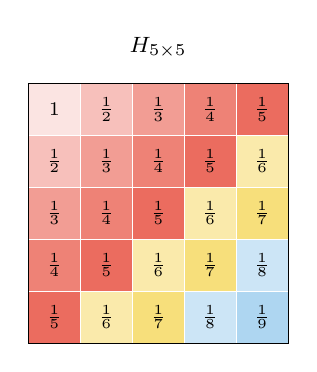
\begin{tikzpicture}[x=0.66cm,y=0.66cm, every node/.style={font=\scriptsize}]
  \def\cell{1}

  % ------------------------------------------------
  % 5x5 Hilbert entries with a simple warm->cool ramp
  % (by diagonal "bands"). Stable + visually clear.
  % ------------------------------------------------

  % Row 0
  \Hcell{0}{0}{Hhot!15}{1}
  \Hcell{0}{1}{Hhot!35}{\tfrac12}
  \Hcell{0}{2}{Hhot!55}{\tfrac13}
  \Hcell{0}{3}{Hhot!70}{\tfrac14}
  \Hcell{0}{4}{Hhot!82}{\tfrac15}

  % Row 1
  \Hcell{1}{0}{Hhot!35}{\tfrac12}
  \Hcell{1}{1}{Hhot!55}{\tfrac13}
  \Hcell{1}{2}{Hhot!70}{\tfrac14}
  \Hcell{1}{3}{Hhot!82}{\tfrac15}
  \Hcell{1}{4}{Hmid!35}{\tfrac16}

  % Row 2
  \Hcell{2}{0}{Hhot!55}{\tfrac13}
  \Hcell{2}{1}{Hhot!70}{\tfrac14}
  \Hcell{2}{2}{Hhot!82}{\tfrac15}
  \Hcell{2}{3}{Hmid!35}{\tfrac16}
  \Hcell{2}{4}{Hmid!55}{\tfrac17}

  % Row 3
  \Hcell{3}{0}{Hhot!70}{\tfrac14}
  \Hcell{3}{1}{Hhot!82}{\tfrac15}
  \Hcell{3}{2}{Hmid!35}{\tfrac16}
  \Hcell{3}{3}{Hmid!55}{\tfrac17}
  \Hcell{3}{4}{Hcool!25}{\tfrac18}

  % Row 4
  \Hcell{4}{0}{Hhot!82}{\tfrac15}
  \Hcell{4}{1}{Hmid!35}{\tfrac16}
  \Hcell{4}{2}{Hmid!55}{\tfrac17}
  \Hcell{4}{3}{Hcool!25}{\tfrac18}
  \Hcell{4}{4}{Hcool!40}{\tfrac19}

  % Outline box perfectly aligned to the 5x5 grid
  \draw[black] (0,0) rectangle (5,-5);

  % Label above matrix
  \node[font=\footnotesize] at (2.5,0.7) {$H_{5\times5}$};
\end{tikzpicture}

\vspace{0.25em}
{\footnotesize Larger entries cluster near the top-left.}

\end{column}

\end{columns}
\end{frame}
% -------------------------------------------------
% -------------------------------------------------
\begin{frame}{Why the Hilbert Matrix Matters}
\begin{itemize}
\item Appears harmless
\item Defeats standard numerical solvers
\item Demonstrates limits of floating-point arithmetic
\end{itemize}
\end{frame}

% ———————————————––
\begin{frame}{Notebook Demonstration}
In the accompanying notebook, we:
\begin{itemize}
\item Construct Hilbert matrices of increasing size
\item Solve linear systems numerically
\item Observe loss of accuracy
\end{itemize}

\vspace{1em}
\begin{block}{Key Observation}
As matrix size increases, numerical reliability collapses.
\end{block}
\end{frame}

% ———————————————––
\begin{frame}{What Went Wrong?}
\begin{itemize}
\item The mathematical problem is well defined
\item The algorithm is correct
\item Floating-point arithmetic limits accuracy
\end{itemize}

\vspace{1em}
\begin{alertblock}{Critical Lesson}
The computer did not fail — the mathematics did.
\end{alertblock}
\end{frame}

% ———————————————––
\begin{frame}{Implications for This Course}
\begin{itemize}
\item Matrix structure matters
\item Solver choice matters
\item Blind trust in numerical output is dangerous
\end{itemize}

\vspace{1em}
These themes will reappear throughout the semester.
\end{frame}

% ———————————————––
\begin{frame}{Looking Ahead}
In upcoming lectures, we will:
\begin{itemize}
\item Define condition numbers formally
\item Study direct and iterative solvers
\item Connect conditioning to stiffness matrices
\item Develop strategies for numerical robustness
\end{itemize}
\end{frame}

% ———————————————––
\begin{frame}{Summary}
\begin{itemize}
\item A correct Python setup is essential
\item Matrix algebra underpins computational mechanics
\item Numerical instability is unavoidable but manageable
\end{itemize}

\vspace{1em}
\begin{block}{Next Step}
Work through the Hilbert matrix notebook carefully.
\end{block}
\end{frame}

\end{document}